%TeX

\documentclass{beamer}

\usepackage{graphicx}
\graphicspath{{include/images/}}
\usepackage{verbatim}
\usepackage{xspace}
\usepackage{readarray}
\usepackage{environ}
\usepackage{tikz}
\usepackage{ragged2e}

% just for the vaporsec text
\usepackage{xeCJK}

% \usetheme{DarkConsole}
\usetheme{Madrid}
\useinnertheme{rectangles}
\setbeamercolor{normal text}{bg=black!05}

\newcommand{\VaporSec}{
    \symbol{65334}\symbol{65313}\symbol{65328}\symbol{65327}\symbol{65330}%
    \symbol{65331}\symbol{65317}\symbol{65315}
}

\newcommand{\Aesthetic}{
    \symbol{65313}\symbol{65317}\symbol{65331}\symbol{65332}\symbol{65320}%
    \symbol{65317}\symbol{65332}\symbol{65321}\symbol{65315}
}

\newcommand{\Aesthetics}{\Aesthetic\symbol{65331}}

\title{For Realz Mode!}
\subtitle{
    Reversing an MBR from the CSAW CTF\\
    {\em (and how to write a keygen with a SAT solver)}
}
\author{t0x0 \and @numinit}
\institute{\VaporSec}
\date{2017-10-11}

\begin{document}

\begin{frame}
    \titlepage
\end{frame}

%TeX

\section{Introduction}

\begin{frame}{About us}
    \begin{itemize}
        \item Morgan (@numinit)
        \begin{itemize}
            \item Software developer by day
            \item Tinkerer on everything by night
            \item First Def Con and Toorcon experiences this year
            \item Doing CSAW CTF for a while
        \end{itemize}
        \item t0x0 (@t0x0pg)
        \begin{itemize}
            \item Writes lots of interpreted code
            \item Lives mostly in Windows world
            \item Jack of all trades, master of none (so far)
            \item Obsessively curious
        \end{itemize}
    \end{itemize}
\end{frame}

\begin{frame}{What's CSAW?}
    \begin{columns}
        \column{0.5\textwidth}
        An annual security capture the flag run by New York Polytechnic that
        contains challenges with a \alert{wide range of difficulties},
        attracting everyone from undergraduates to well-known teams

        \column{0.5\textwidth}
        \Graphic{csaw-logo} \\
        \Graphic{scoreboard}
    \end{columns}
\end{frame}

\begin{frame}{What's a security capture the flag?}
    \begin{itemize}
        \item<1-> 48 hours of caffeinated reverse engineering and exploitation
        \item<2-> More seriously: an event where you break a bunch of programs
                  to retrieve hidden strings of text (the flags)
        \item<3-> An opportunity to learn new things - we wouldn't
                  even be presenting if it wasn't for this CTF
    \end{itemize}
\end{frame}

\begin{frame}{Who are \VaporSec?}
    \begin{itemize}
        \item A new \Aesthetic San Diego CTF team
        \item Had 10 participants during the CSAW CTF
        \item Achieved 15th in CSAW industry professional bracket, not bad for
              the first time
    \end{itemize}
\end{frame}

%TeX

\section{Reversing the MBR}

\begin{frame}{RE400 what?\ldots}
    \begin{columns}
        \column{0.5\textwidth}
	        \begin{itemize}
                \item Challenge worth 400 points
                \item Reverse Engineering category
                \item We get some hints right away\ldots
                \begin{itemize}
                	\item This is an MBR
                	\item \ldots from an x86 system
        	    \end{itemize}
            \end{itemize}
        \column{0.5\textwidth}
                {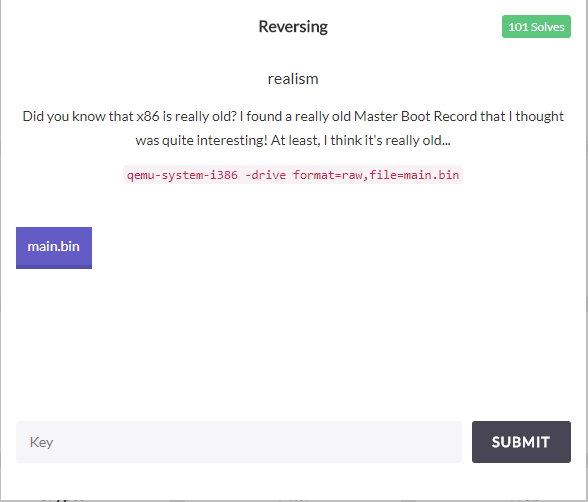
\includegraphics[width=\textwidth]{re400}}
    \end{columns}
\end{frame}

\begin{frame}{A place to start\ldots}
    \begin{columns}
        \column{0.5\textwidth}
	        \begin{itemize}
                \item<1-> Wikipedia, of course!
		        \begin{itemize}
    	            \item<2-> 512 bytes
        	        \item<2-> MBR signature: 55 AA
            	    \item<2-> "expected to contain real mode machine language instructions"
                	\item<2-> little-endian
                	\item<2-> loads at 0000:7C00
	            \end{itemize}                	
            \end{itemize}
        \column{0.5\textwidth}
                {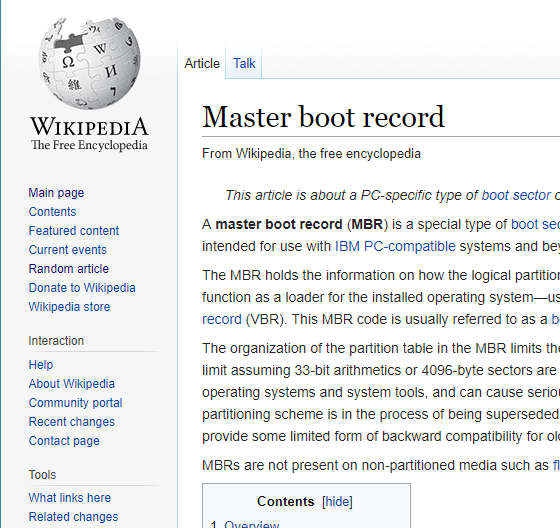
\includegraphics[width=\textwidth]{wikimbr}}
    \end{columns}
\end{frame}

\begin{frame}{Tool Time!\ldots}
    \framesubtitle{qemu (gift wrapped)}
    \begin{columns}
        \column{0.5\textwidth}
            \only<1> {
              	\begin{itemize}
             		\item -s (gdb)
                	\item -S (suspend)
        	       	\item -vnc:1
	            \end{itemize}
            }
            \only<2> {
             	\begin{itemize}
            		\item QEMU/Monitor
              		\begin{itemize}
	    	        	\item info registers
    	    	       	\item system reset
    	    	    \end{itemize}
        	    \end{itemize}
        	}
        \column{0.5\textwidth}
            \only<1>{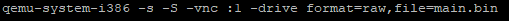
\includegraphics[width=\textwidth]{launch-qemu}\newline\newline
            		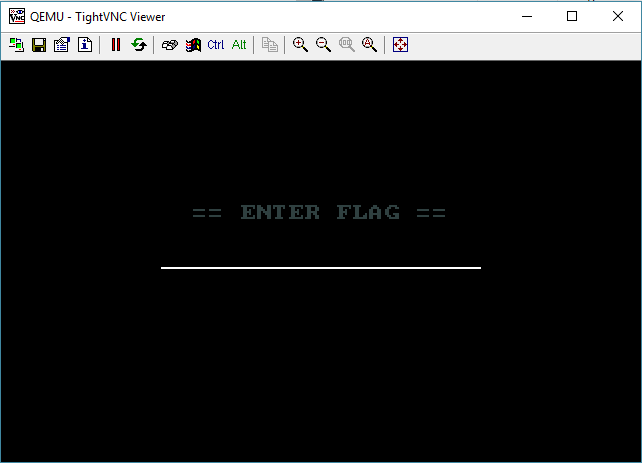
\includegraphics[width=\textwidth]{qemu-vnc}
			}
            \only<2>{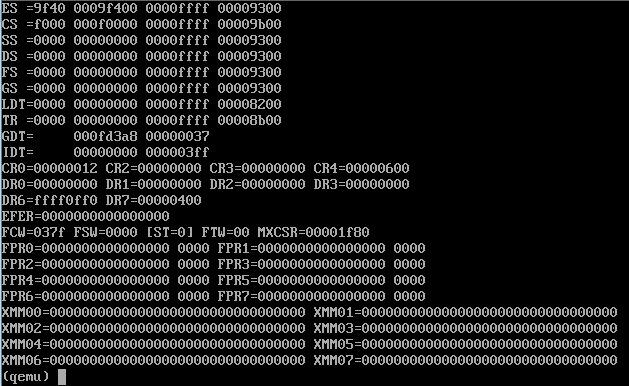
\includegraphics[width=\textwidth]{qemu-info-registers-1}}
    \end{columns}
\end{frame}

\begin{frame}{Tool Time!\ldots}
    \framesubtitle{gdb}
    \begin{columns}
        \column{0.5\textwidth}
                \begin{itemize}
                	\only<1>{
						\item target remote localhost:1234
						\item set architecture i8086
							(bootloaders are 16 bit, right?)
						\item display/i \$pc - print program counter
						\item br *0xADDR - set breakpoint
						\item si - run one instruction
						\item c - continue
					}
					\only<2->{
						\item info reg
						\uncover<3->{\item info frame}
						\uncover<4->{\item x /CT 0xADDR - display C units of T type from ADDR
									\item set {int}0xADDR = 42
									\item set {char[4]} 0xADDR = "AAA"
						}
					}
				\end{itemize}
		\column{0.5\textwidth}
				\only<1>{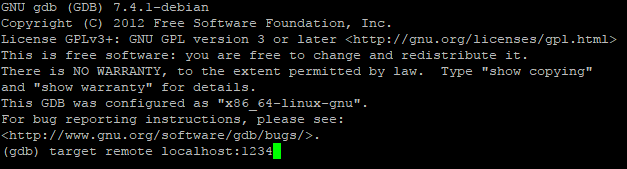
\includegraphics[width=\textwidth]{launch-gdb}\newline\newline
						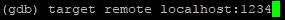
\includegraphics[width=\textwidth]{gdb-target}}
				\only<2>{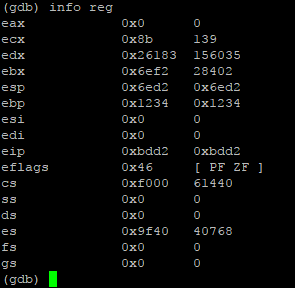
\includegraphics[width=\textwidth]{gdb-info-reg-1}}
				\only<3>{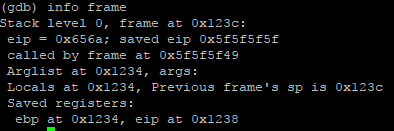
\includegraphics[width=\textwidth]{gdb-info-frame}}
				\only<4-5>{
					\uncover<4->{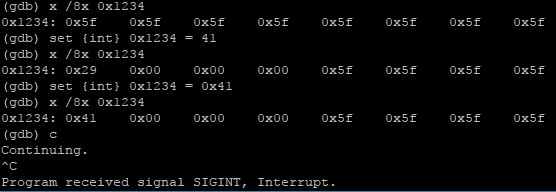
\includegraphics[width=\textwidth]{gdb-x-set-1}}
					\uncover<5->{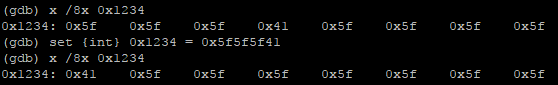
\includegraphics[width=\textwidth]{gdb-x-set-2}}
				}
				\only<6>{
					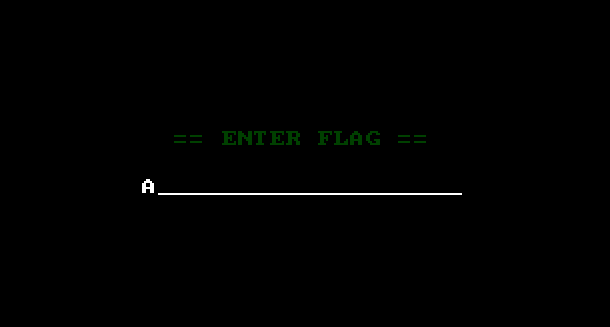
\includegraphics[width=\textwidth]{after-set}
				}
	\end{columns}
\end{frame}
%include{include/part2}

\end{document}
